\PassOptionsToPackage{unicode=true}{hyperref} % options for packages loaded elsewhere
\PassOptionsToPackage{hyphens}{url}
\PassOptionsToPackage{dvipsnames,svgnames*,x11names*}{xcolor}
%
\documentclass[,french]{article}
\usepackage{lmodern}
\usepackage{amssymb,amsmath}
\usepackage{ifxetex,ifluatex}
\usepackage{fixltx2e} % provides \textsubscript
\ifnum 0\ifxetex 1\fi\ifluatex 1\fi=0 % if pdftex
  \usepackage[T1]{fontenc}
  \usepackage[utf8]{inputenc}
  \usepackage{textcomp} % provides euro and other symbols
\else % if luatex or xelatex
  \usepackage{unicode-math}
  \defaultfontfeatures{Ligatures=TeX,Scale=MatchLowercase}
\fi
% use upquote if available, for straight quotes in verbatim environments
\IfFileExists{upquote.sty}{\usepackage{upquote}}{}
% use microtype if available
\IfFileExists{microtype.sty}{%
\usepackage[]{microtype}
\UseMicrotypeSet[protrusion]{basicmath} % disable protrusion for tt fonts
}{}
\IfFileExists{parskip.sty}{%
\usepackage{parskip}
}{% else
\setlength{\parindent}{0pt}
\setlength{\parskip}{6pt plus 2pt minus 1pt}
}
\usepackage{xcolor}
\usepackage{hyperref}
\hypersetup{
            pdftitle={Itinéraire entre deux stations du métro parisien},
            pdfauthor={Kim Antunez et Alain Quartier-la-Tente},
            colorlinks=true,
            linkcolor=Maroon,
            filecolor=Maroon,
            citecolor=Blue,
            urlcolor=blue,
            breaklinks=true}
\urlstyle{same}  % don't use monospace font for urls
\usepackage[margin=1in]{geometry}
\usepackage{graphicx,grffile}
\makeatletter
\def\maxwidth{\ifdim\Gin@nat@width>\linewidth\linewidth\else\Gin@nat@width\fi}
\def\maxheight{\ifdim\Gin@nat@height>\textheight\textheight\else\Gin@nat@height\fi}
\makeatother
% Scale images if necessary, so that they will not overflow the page
% margins by default, and it is still possible to overwrite the defaults
% using explicit options in \includegraphics[width, height, ...]{}
\setkeys{Gin}{width=\maxwidth,height=\maxheight,keepaspectratio}
\setlength{\emergencystretch}{3em}  % prevent overfull lines
\providecommand{\tightlist}{%
  \setlength{\itemsep}{0pt}\setlength{\parskip}{0pt}}
\setcounter{secnumdepth}{5}
% Redefines (sub)paragraphs to behave more like sections
\ifx\paragraph\undefined\else
\let\oldparagraph\paragraph
\renewcommand{\paragraph}[1]{\oldparagraph{#1}\mbox{}}
\fi
\ifx\subparagraph\undefined\else
\let\oldsubparagraph\subparagraph
\renewcommand{\subparagraph}[1]{\oldsubparagraph{#1}\mbox{}}
\fi

% set default figure placement to htbp
\makeatletter
\def\fps@figure{htbp}
\makeatother

\usepackage{etoolbox}
\makeatletter
\providecommand{\subtitle}[1]{% add subtitle to \maketitle
  \apptocmd{\@title}{\par {\large #1 \par}}{}{}
}
\makeatother
\usepackage{pdflscape}
\newcommand{\blandscape}{\begin{landscape}}
\newcommand{\elandscape}{\end{landscape}}
\usepackage{fontawesome5}
\usepackage{caption}
% https://github.com/rstudio/rmarkdown/issues/337
\let\rmarkdownfootnote\footnote%
\def\footnote{\protect\rmarkdownfootnote}

% https://github.com/rstudio/rmarkdown/pull/252
\usepackage{titling}
\setlength{\droptitle}{-2em}

\pretitle{\vspace{\droptitle}\centering\huge}
\posttitle{\par}

\preauthor{\centering\large\emph}
\postauthor{\par}

\predate{\centering\large\emph}
\postdate{\par}
\ifnum 0\ifxetex 1\fi\ifluatex 1\fi=0 % if pdftex
  \usepackage[shorthands=off,main=]{babel}
\else
  % load polyglossia as late as possible as it *could* call bidi if RTL lang (e.g. Hebrew or Arabic)
  \usepackage{polyglossia}
  \setmainlanguage[]{}
\fi

\title{Itinéraire entre deux stations du métro parisien}
\author{Kim Antunez et Alain Quartier-la-Tente}
\date{07/01/2020 - 15h30 à 15h45}

\begin{document}
\maketitle

{
\hypersetup{linkcolor=}
\setcounter{tocdepth}{2}
\tableofcontents
}
\hypertarget{introduction}{%
\section{Introduction}\label{introduction}}

Ce rapport décrit le projet C++ de Kim Antunez et d'Alain
Quartier-la-Tente dont l'objectif est de permettre à l'utilisateur
d'obtenir un chemin entre deux stations de métro selon deux critères :
le plus court chemin ou le chemin avec le moins de correspondances.
L'ensemble des données et des codes utilisés sont disponibles sous
\url{https://github.com/AQLT/Metro_Cpp}, la section
\ref{sec:pris_en_main} décrivant comment prendre en main et utiliser
l'application. Les données utilisées sont les données du métro parisien
fournies par la RATP (section \ref{sec:def_donnees}), l'implémentation
des classes est décrite dans la section \ref{sec:desc_classes},
l'algorithme utilisé pour calculer les chemins est l'algorithme de
Dijkstra (section \ref{sec:algo}). Enfin, les pistes d'amélioration sont
décrites dans la partie \ref{sec:amelioration}.

Pour mieux se retrouver dans le réseau parisien, le plan de l'ensemble
des lignes a été rajouté dans la section \ref{sec:lignes_metro}.

\hypertarget{sec:pris_en_main}{%
\section{Prise en main du programme}\label{sec:pris_en_main}}

\hypertarget{sec:def_donnees}{%
\section{Description des données}\label{sec:def_donnees}}

\hypertarget{description-des-donnuxe9es-uxe0-disposition}{%
\subsection{Description des données à
disposition}\label{description-des-donnuxe9es-uxe0-disposition}}

Toutes les données utilisées dans ce projet sont issues de la RATP de la
base \texttt{offre-transport-de-la-ratp-format-gtfs}
(\url{https://dataratp.opendatasoft.com/explore/dataset/offre-transport-de-la-ratp-format-gtfs/information/}).
Ces données sont au format \emph{General Transit Feed Specification}
(GTFS) qui est un format standardisé pour publier un réseau de transport
en commun (horaires, informations géographiques, etc.).

Pour les données de la RATP sont disponibles sous deux formes d'archives
:

\begin{itemize}
\tightlist
\item
  Une archive avec des fichiers GTFS réparties par lignes ;\\
\item
  Une archive avec des fichiers GTFS pour l'ensemble du réseau (métro,
  bus, tram et RER).
\end{itemize}

C'est cette première archive que nous avons utilisé pour nous
restreindre plus facilement aux données des lignes de métro uniquement.
Nous avons stockés les données utilisées ici :
\url{https://github.com/AQLT/Metro_Cpp/tree/master/Data}.

Pour chaque ligne, les données sont stockées dans différents fichiers :

\begin{enumerate}
\def\labelenumi{\arabic{enumi}.}
\item
  \texttt{routes.txt} : définit les itinéraires des transports en commun
  \(\rightarrow\) données \textbf{utilisées} avec le fichier
  \texttt{trips.txt} pour identifier l'ordre de passage à chaque arrêt
  pour les lignes aller et retour.
\item
  \texttt{stops.txt} : définit l'ensemble des arrêts où les usages
  peuvent monter ou descendre, avec le nom de l'arrêt, l'adresse et les
  coordonnées GPS \(\rightarrow\) données \textbf{utilisées} dans ce
  projet pour définir l'ensemble des arrêts.
\item
  \texttt{stop\_times.txt} : définit, pour chaque trajet et pour chaque
  arrêt, les heures d'arrivée et de départ du métro \(\rightarrow\)
  données \textbf{utilisées} avec le fichier \texttt{trip.txt} pour
  connaître le temps de trajet entre deux stations de la même ligne.
\item
  \texttt{transfers.txt} : définit les règles de liaison aux pôles de
  correspondance entre des itinéraires \(\rightarrow\) données
  \textbf{utilisées} dans ce projet pour connaître les correspondances
  et les temps de correspondance entre les lignes.
\item
  \texttt{trips.txt} : définit l'ensemble des trajets pour chaque ligne
  (i.e. : tous les trajets prévus dans la journée) \(\rightarrow\)
  données \textbf{utilisées} avec le fichier \texttt{routes.txt} et
  \texttt{stop\_times.txt} pour identifier pour chaque ligne l'ordre de
  passage et le temps de trajet entre chaque arrêt \footnote{Dans ce
    projet nous ne prenons pas en compte l'heure à laquelle la recherche
    d'itinéraire a été faite : pour chaque ``route'' un seul ``trip'' a
    donc été utilisé}.
\item
  \texttt{calendar\_dates.txt} : définit les exceptions pour les
  services définis dans le fichier \texttt{calendar.txt} \(\rightarrow\)
  données \textbf{non utilisées} dans ce projet.
\item
  \texttt{calendar.txt} : définit les dates auxquelles le service est
  disponible pour des itinéraires spécifiques selon un calendrier
  hebdomadaire. Ce fichier spécifie les dates de début et de fin du
  service, ainsi que les jours de la semaine où le service est
  disponible \(\rightarrow\) données \textbf{non utilisées} dans ce
  projet.
\item
  \texttt{agency.txt} : définit une ou plusieurs agences de transports
  publics dont les services sont représentés dans l'ensemble de données
  \(\rightarrow\) données \textbf{non utilisées} dans ce projet.
\end{enumerate}

Plus d'informations sur les données GTFS sont disponibles sur le site de
Google : \url{https://developers.google.com/transit/gtfs/reference/}.

\hypertarget{difficultuxe9s-et-solutions-adoptuxe9es}{%
\subsection{Difficultés et solutions
adoptées}\label{difficultuxe9s-et-solutions-adoptuxe9es}}

Chaque arrêt est définit par une identifiant unique et cet identifiant
est différent pour chaque ligne et pour chaque route (aller et retour)
sans qu'aucun temps de correspondance n'ait été définit dans les
données. Certains itinéraires étaient donc impossibles à calculer : par
exemple, si l'on est sur l'arrêt de métro Gaîté sur la ligne 13
direction Châtillon-Montrouge on ne peut rejoindre l'arrêt
Montparnasse.\\
\(\rightarrow\) \textbf{Solution adoptée} : ajouter un temps de
transfert égal à 0 pour chaque arrêt pour passer d'une ligne aller à la
ligne retour et inversement. Ainsi, le temps de transfert est nul pour
passer de l'arrêt de métro Gaîté sur la ligne 13 direction
Châtillon-Montrouge à l'arrêt de métro Gaîté sur la ligne 13 direction
Saint-Denis/Les Courtilles. En revanche cela rend le calcul du temps de
trajet moins fiable pour deux raisons :

\begin{enumerate}
\def\labelenumi{\arabic{enumi}.}
\item
  Le temps de transfert entre deux lignes n'est pas le même en fonction
  de la direction que l'on prend.
\item
  Pour faire certains itinéraires, il est nécessaire de changer de
  direction tout en restant sur la même ligne (par exemple sur la ligne
  13 passer de Guy Môquet à Brochant il faut aller jusqu'à l'arrêt La
  Fourche et changer de direction). Puisque nous n'avons pas pris en
  compte de temps d'attente moyen d'un métro, le temps du trajet est
  sous-estimé.
\end{enumerate}

Cette façon de coder les arrêts implique que certains arrêts ne sont
associés qu'à une ligne (aller ou retour) alors que d'autres sont
associés à deux lignes (par exemple sur la ligne 13 avec 2 lignes aller
ou 2 lignes retour).

Plusieurs incohérences sur les trajets ont également étaient trouvées :

\begin{itemize}
\item
  Le fichier \texttt{routes.txt} ne permettait pas toujours de bien
  identifier les lignes aller et retour. En effet, pour certaines lignes
  de métro, pour le même identifiant de ``trip'' et pour une ``route''
  fixée il pouvait y avoir au même horaire un départ d'un terminus pour
  une direction et du terminus opposé pour l'autre direction. Cela
  devrait normalement être impossible puisque la ``route'' permet
  d'identifier la directement. Ce problème affecté les lignes 1, 4, 7,
  7B et 13 : un travail manuel a donc été fait pour identifier
  correctement les lignes aller et retour.
\item
  Certaines ``routes'' de la base de données n'existent pas en vrai.
  C'est le cas d'une des routes de la ligne 10 ``BOULOGNE - PONT DE
  SAINT CLOUD \textless{}-\textgreater{} GARE D'AUSTERLITZ) - Aller''
  qui partirait de l'arrêt Porte d'Auteuil pour ensuite aller à l'arrêt
  Michel-Ange Molitor et continuer direction Gare D'austerlitz (alors
  que depuis Porte d'Auteuil la seule direction possible est Boulogne).
  Cette ``route'' n'a pas pas été considéré dans notre algorithme.
\end{itemize}

Pour simplifier le chargement des données en C++, nous avons pré-traité
les données dans le logiciel statistique \faRProject :

\begin{itemize}
\item
  Pour chaque ``route'' nous avons créé un fichier avec :

  \begin{itemize}
  \item
    Le fichier \texttt{stops.txt} où on a enlevé les accents (permet de
    créer l'ensemble des arrêts) ;
  \item
    L'ensemble des arrêts de manière ordonnée ainsi que le nom de la
    route (permet de créer toutes les lignes, d'identifier les arrêts
    traversés ainsi que l'ordre de passage).
  \end{itemize}
\item
  Deux matrices carrées ayant autant de colonnes que d'identifiants
  d'arrêts :

  \begin{itemize}
  \item
    \texttt{voisins\_type.txt} : la coordonnée (i,j) vaut -1 si les deux
    arrêts ne sont pas directement connectés, 0 si les deux arrêts sont
    connectés et sont sur la même ligne (i.e. : si ce sont des arrêts
    voisins) et 1 si les deux arrêts sont connectés mais sur deux lignes
    différentes (par exemple entre la ligne 4 et la ligne 13 à l'arrêt
    Montparnasse).
  \item
    \texttt{voisins.txt} : la coordonnée (i,j) correspond au temps
    nécessaire pour aller directement l'arrêt i à l'arrêt j (avec une
    valeur égale à -1 s'il n'y a pas de correspondance directe
    possible).
  \end{itemize}
\end{itemize}

L'ensemble de ces nouveaux fichiés sont stockés sous
\url{https://github.com/AQLT/Metro_Cpp/tree/master/Data\%20projet}.

\hypertarget{sec:desc_classes}{%
\section{Description des classes}\label{sec:desc_classes}}

\hypertarget{sec:algo}{%
\section{Description de l'algorithme}\label{sec:algo}}

\hypertarget{sec:amelioration}{%
\section{Pistes d'amélioration}\label{sec:amelioration}}

\hypertarget{sec:lignes_metro}{%
\section{Lignes de métro}\label{sec:lignes_metro}}

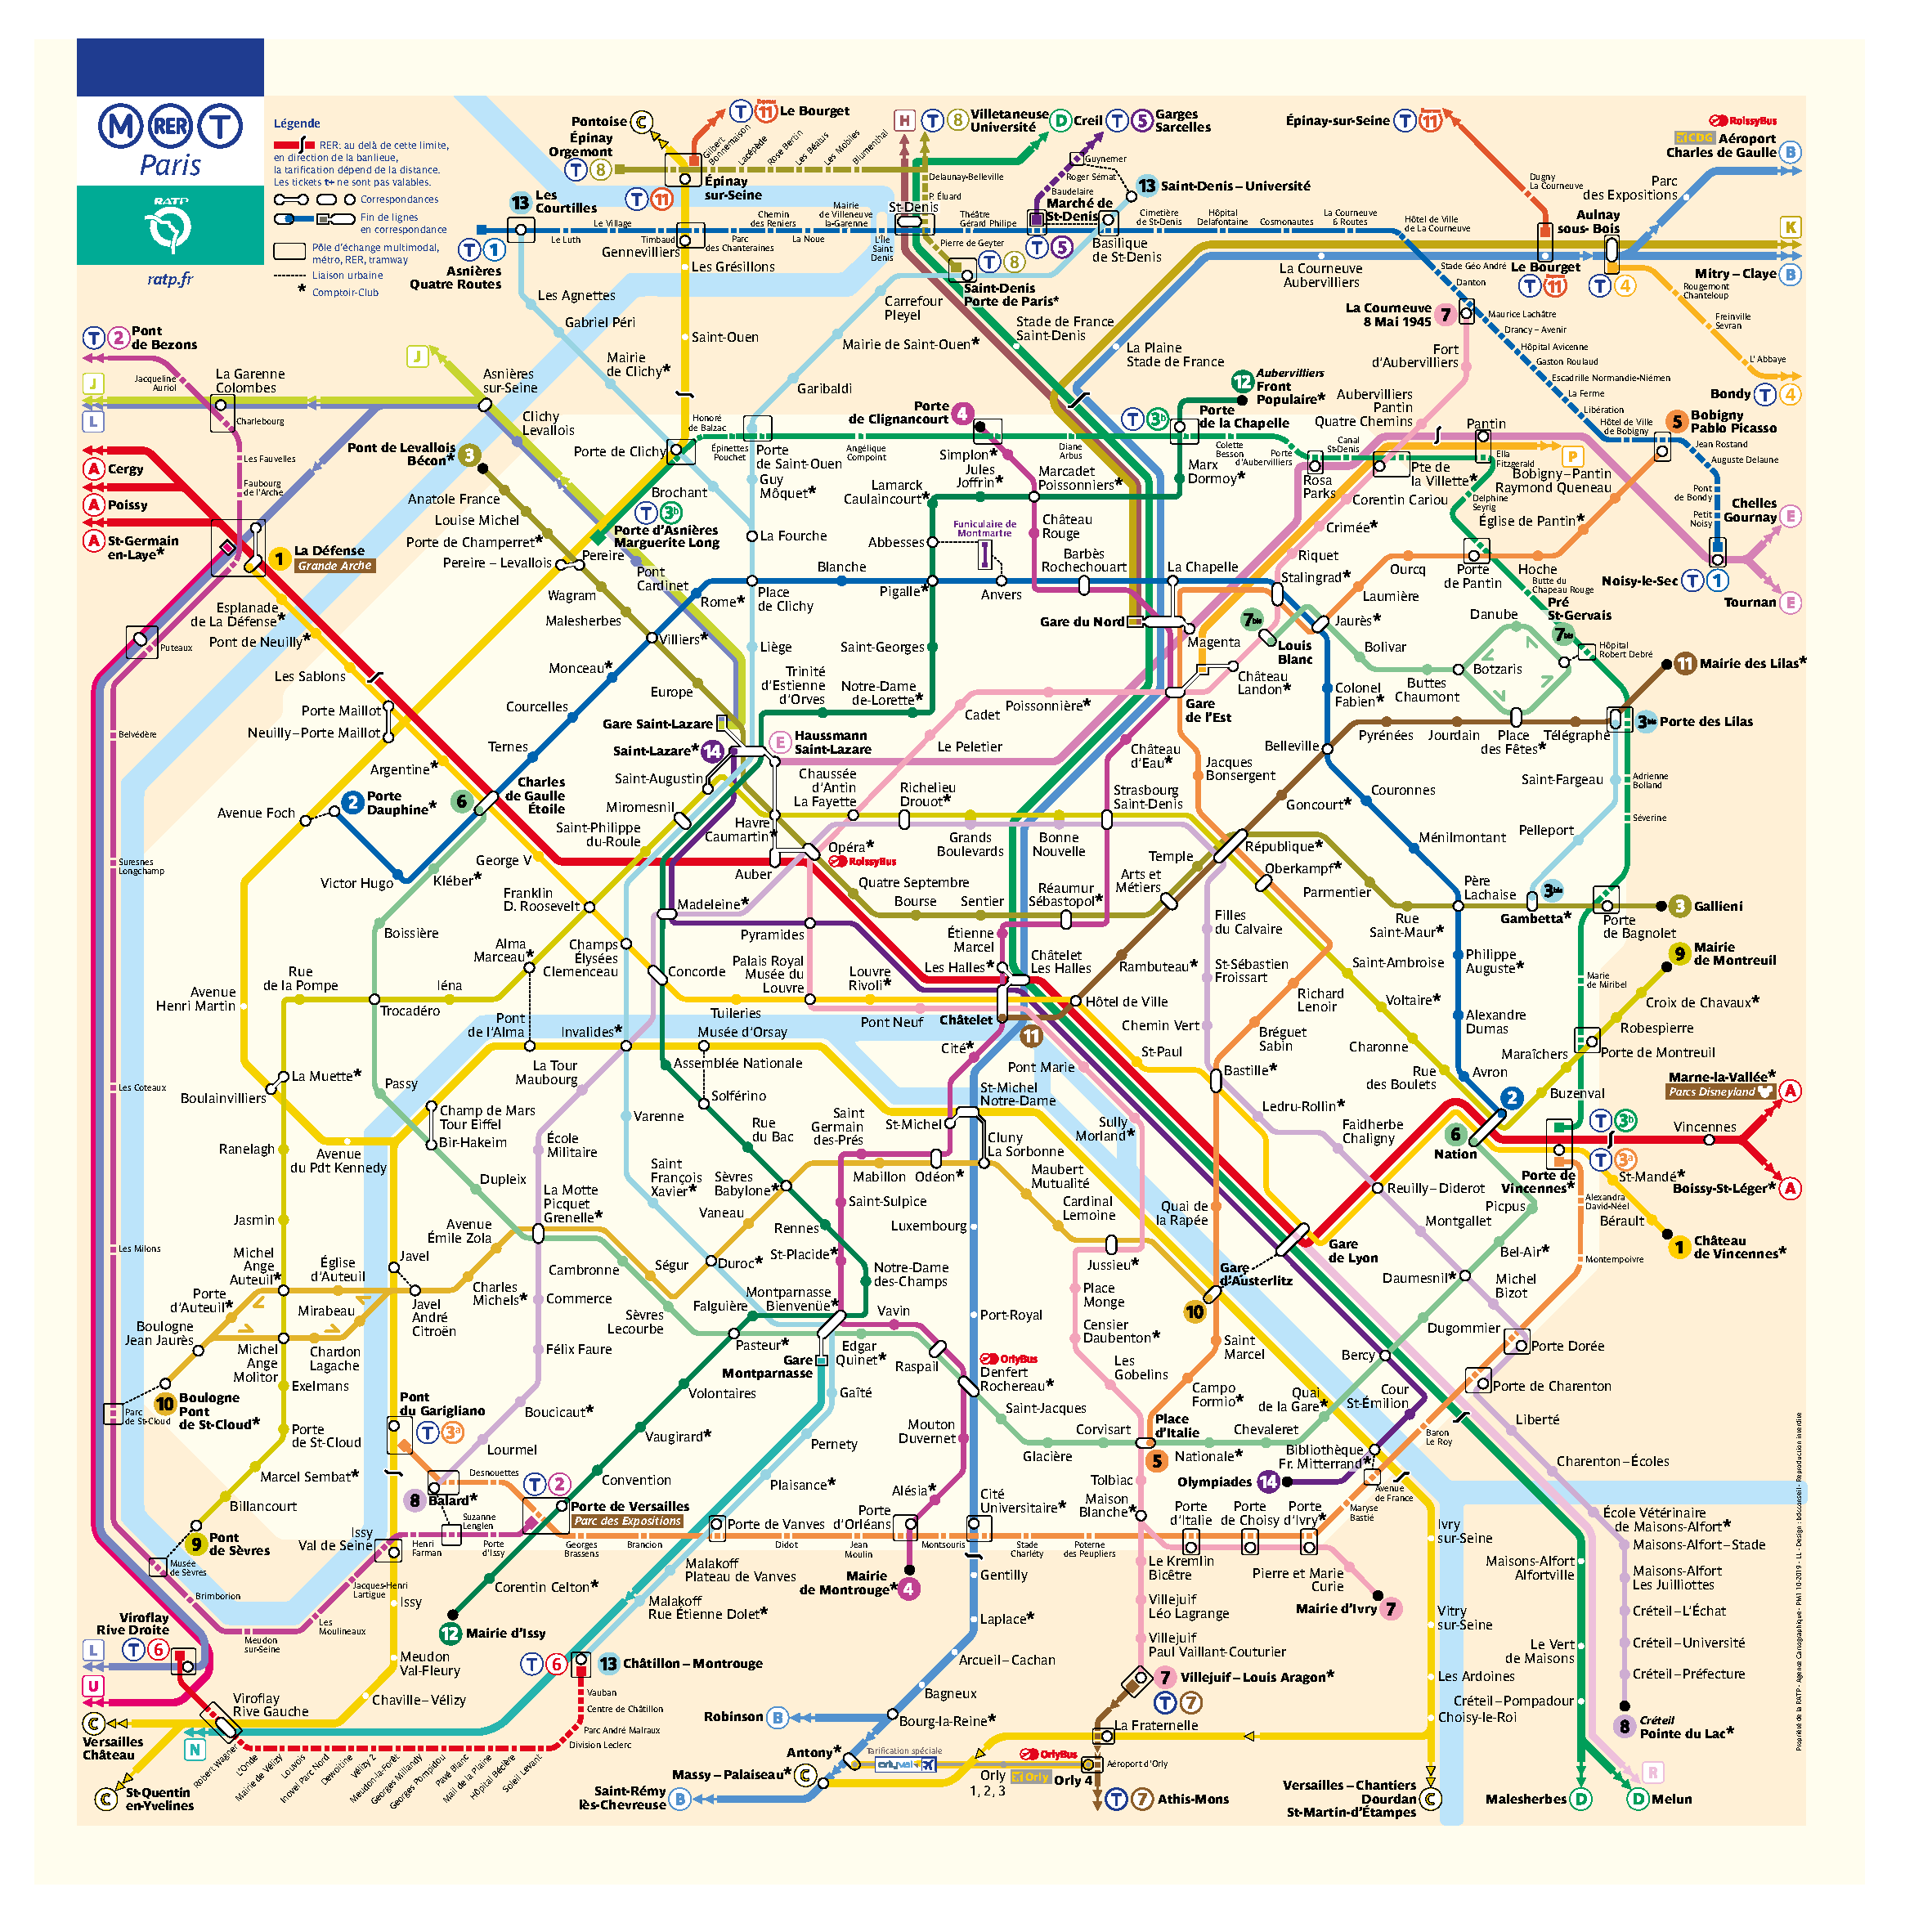
\includegraphics{img/plan_lignes/Plan-Metro.pdf}

\newpage
\begin{landscape}

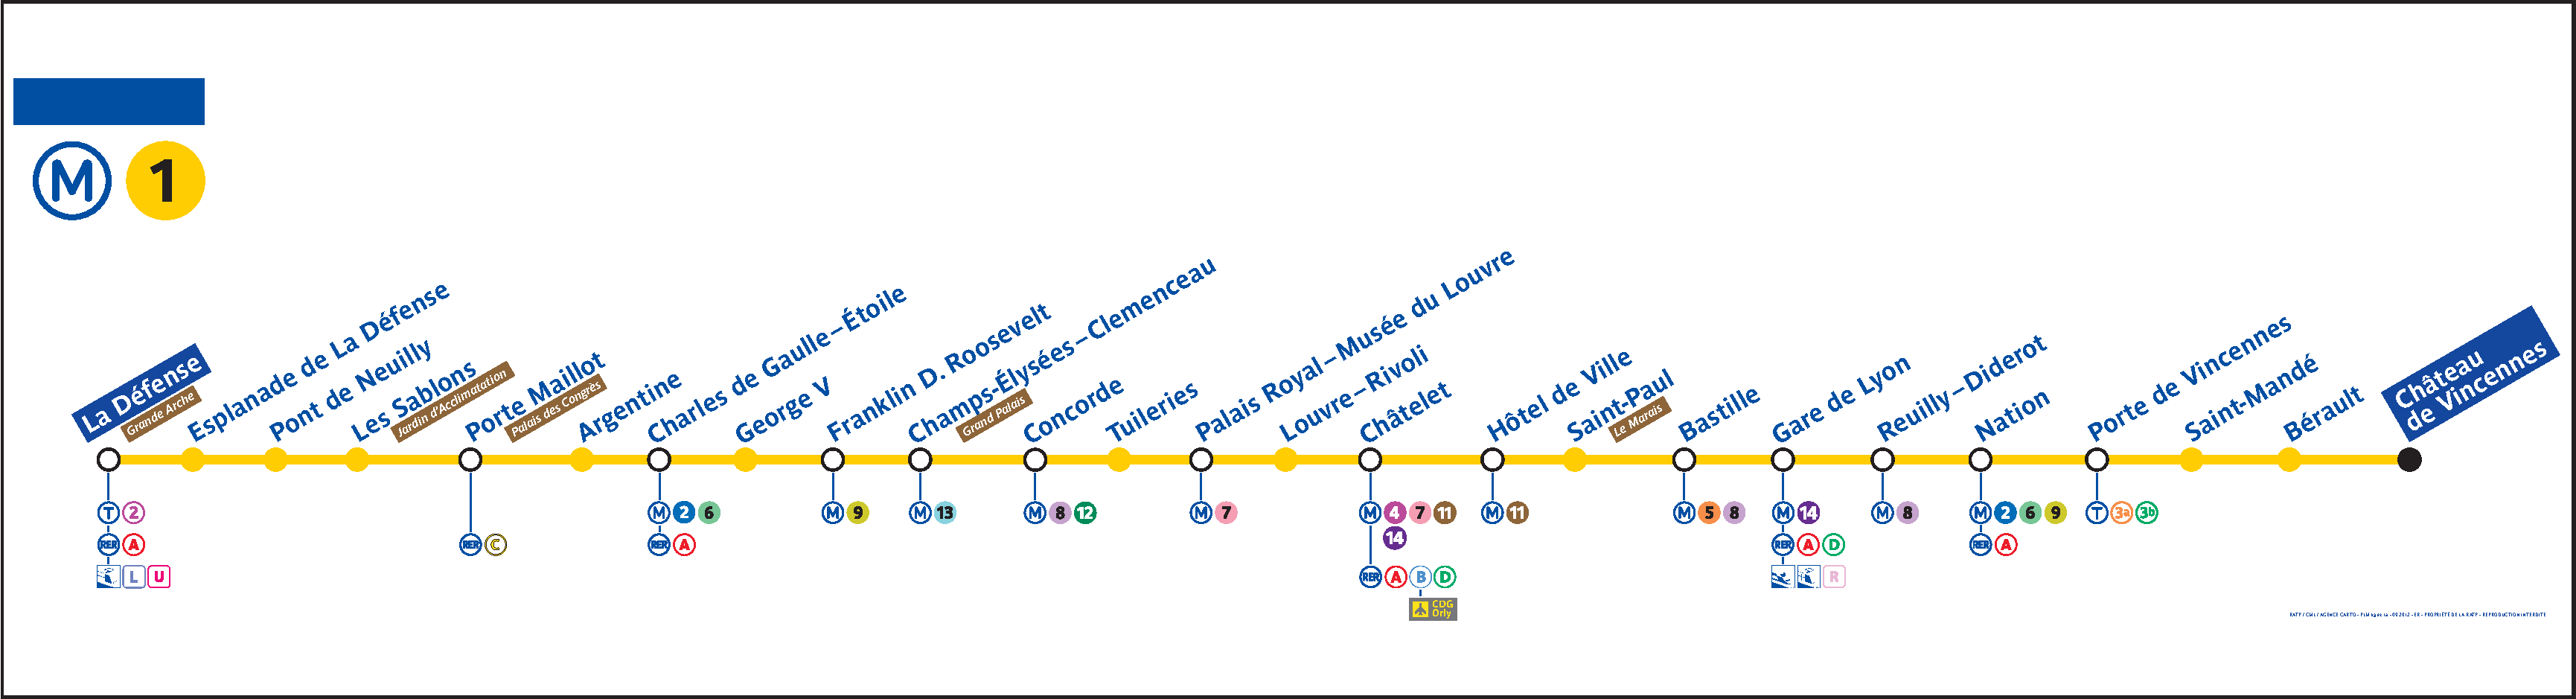
\includegraphics{img/plan_lignes/plan-de-ligne_metro_ligne-1.pdf}

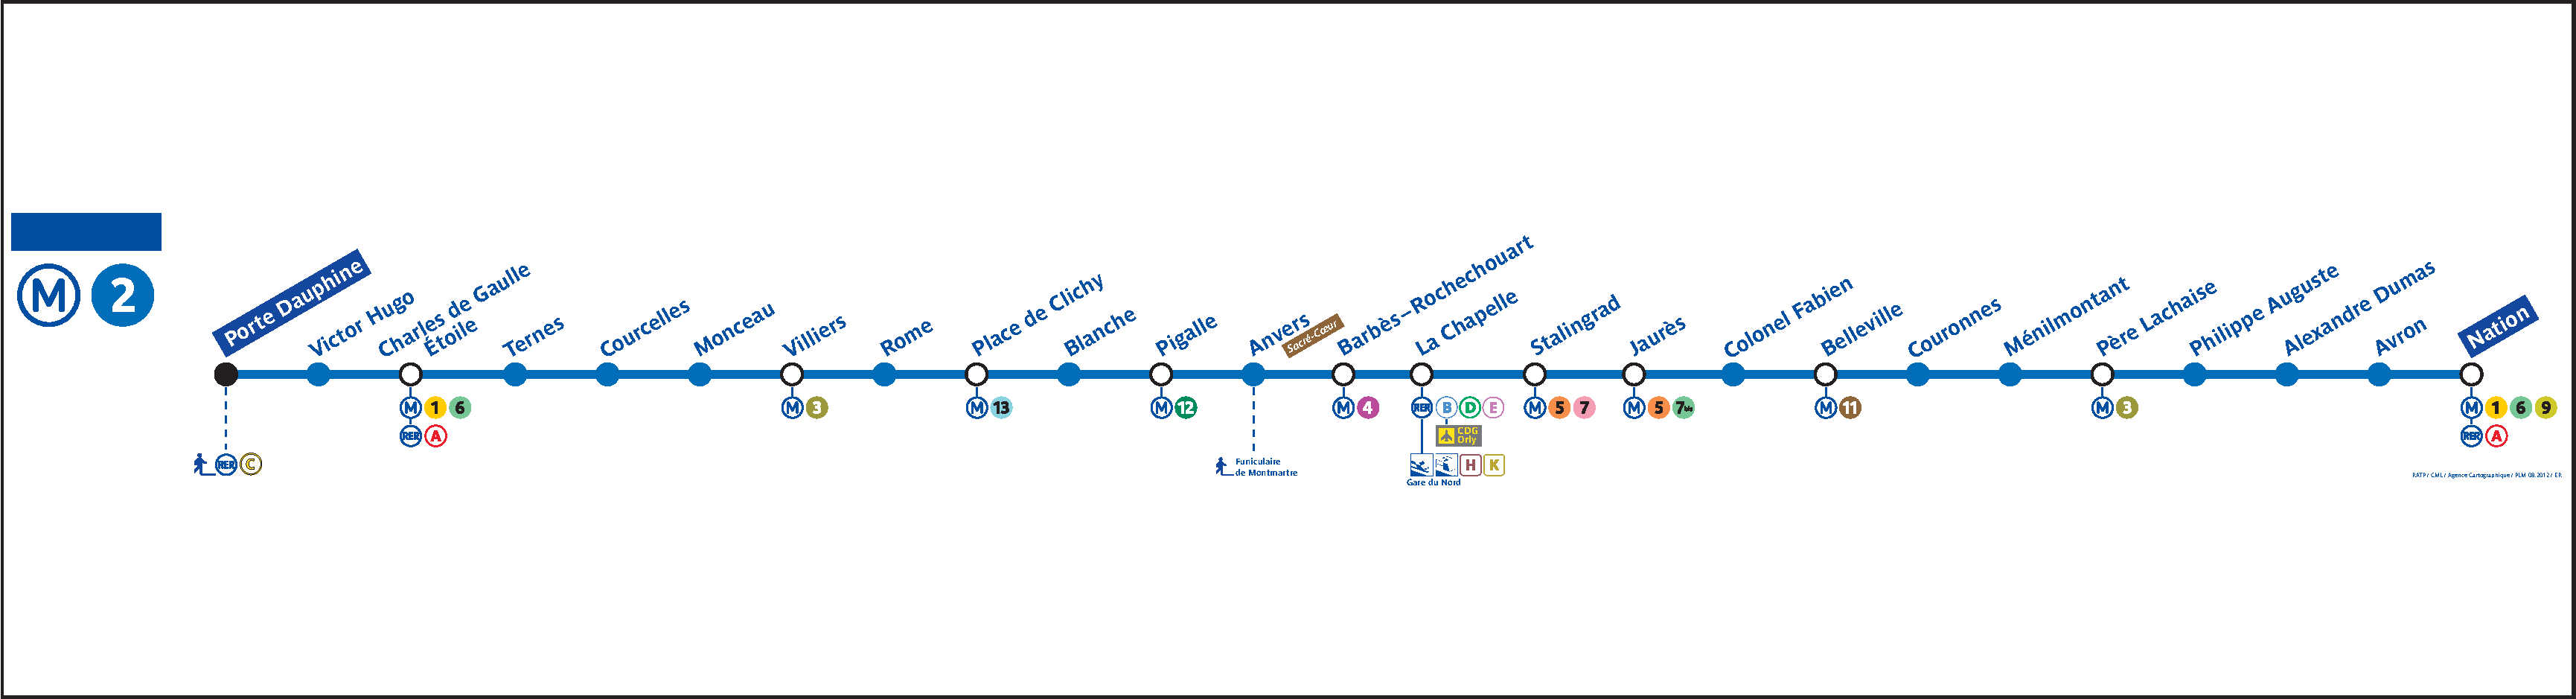
\includegraphics{img/plan_lignes/plan-de-ligne_metro_ligne-2.pdf}

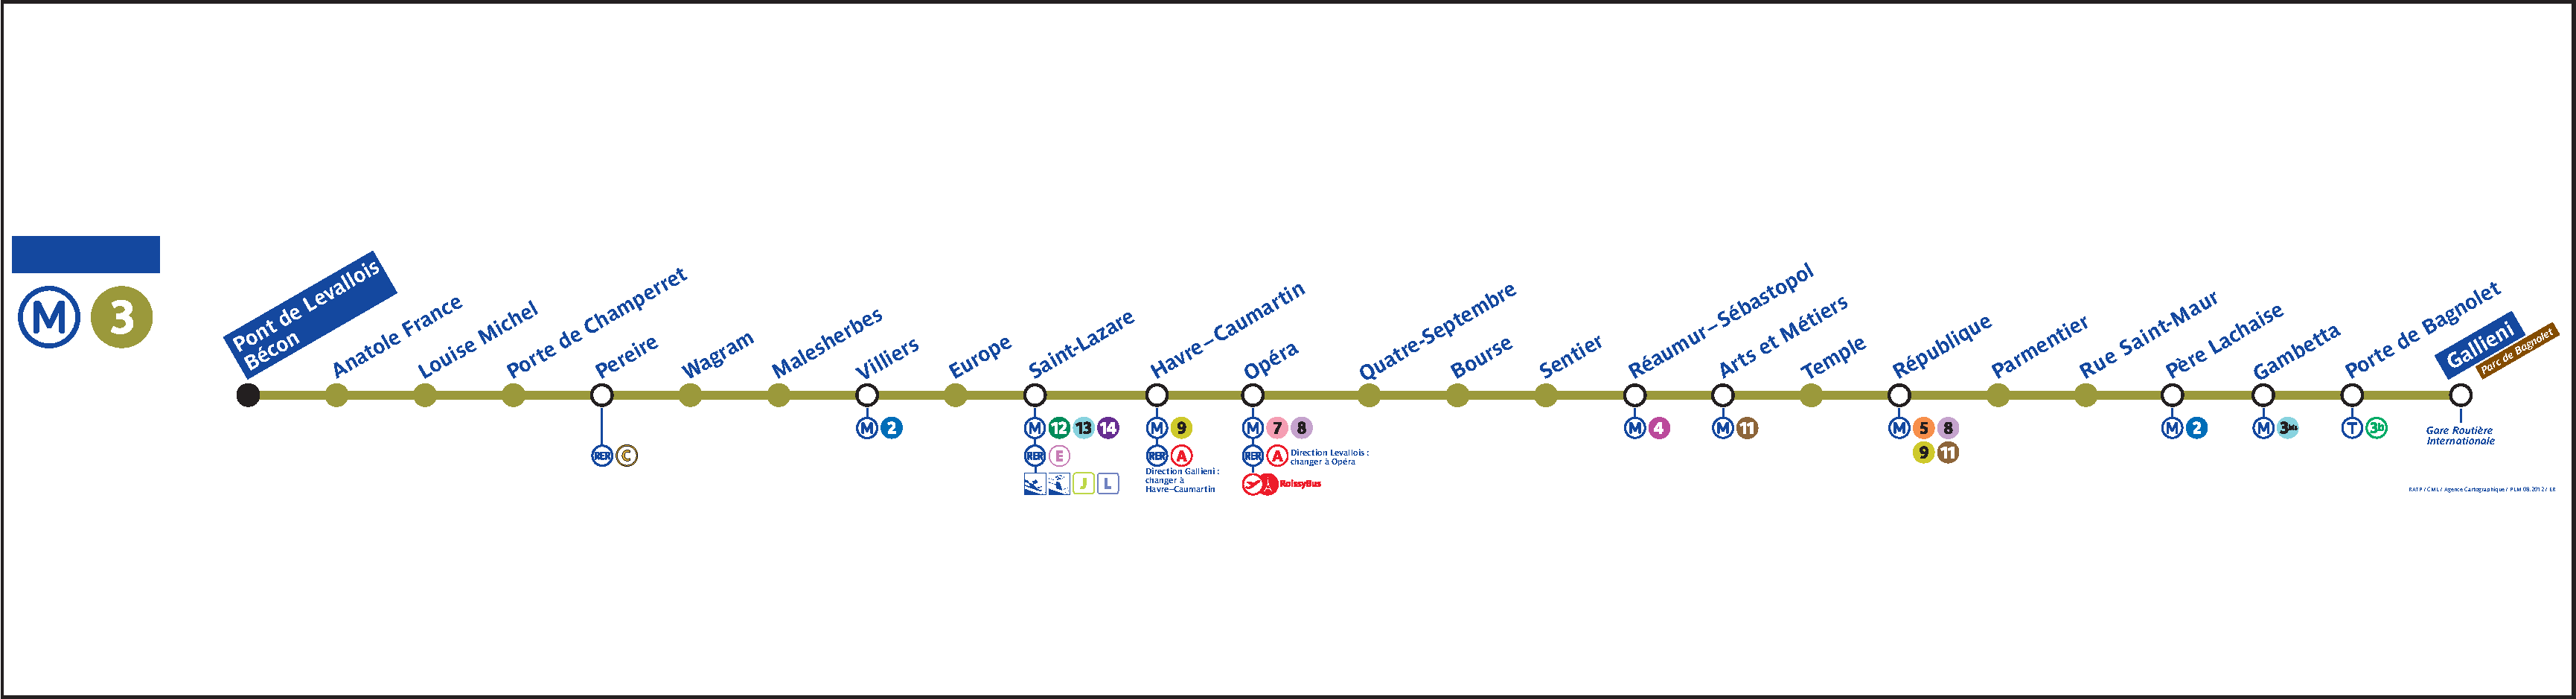
\includegraphics{img/plan_lignes/plan-de-ligne_metro_ligne-3.pdf}

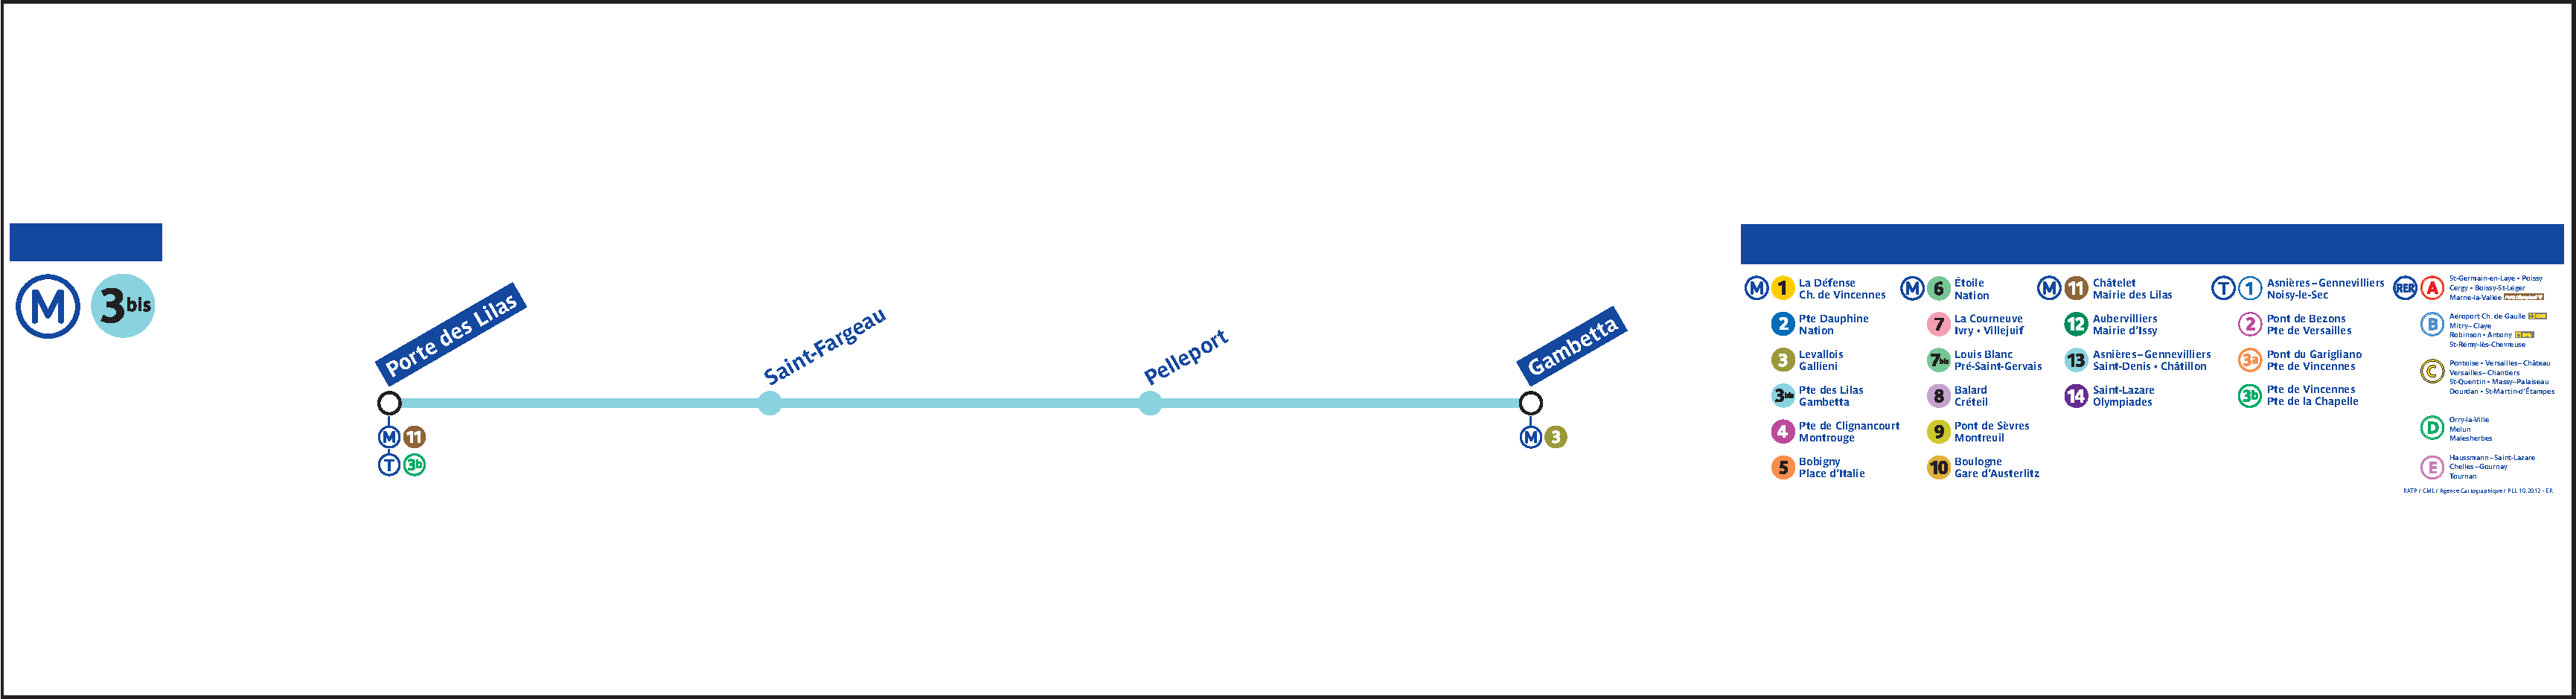
\includegraphics{img/plan_lignes/plan-de-ligne_metro_ligne-3b.pdf}

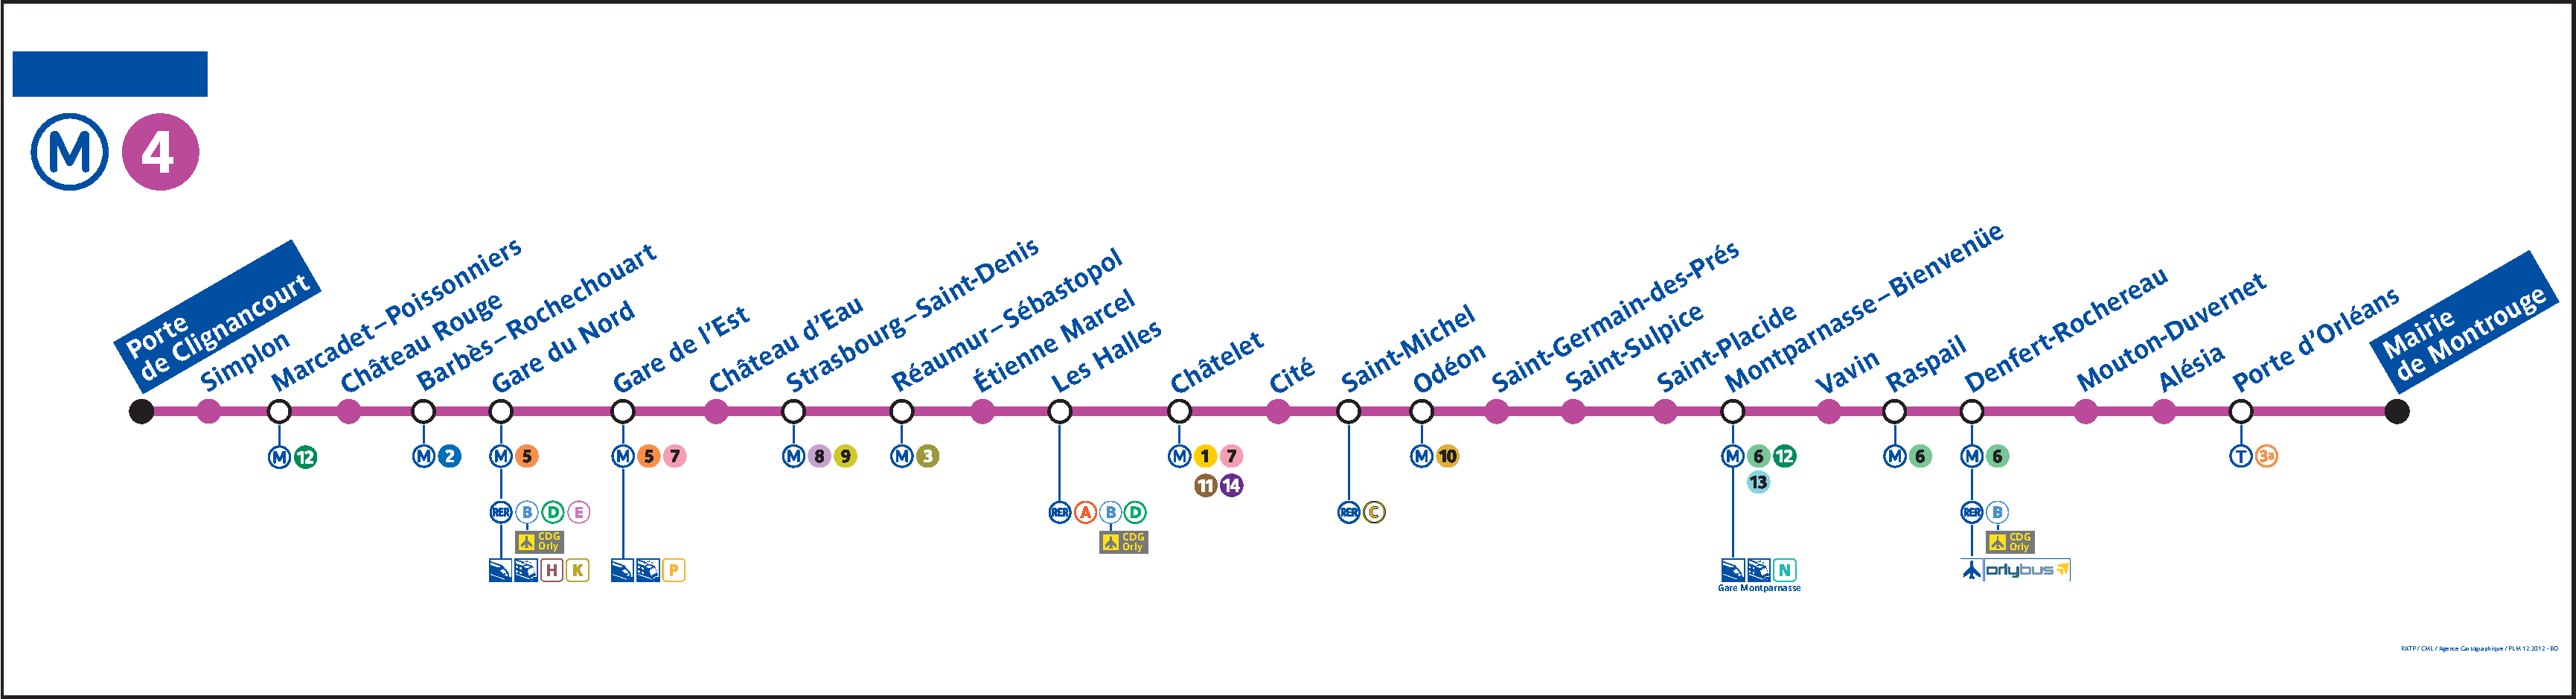
\includegraphics{img/plan_lignes/plan-de-ligne_metro_ligne-4.pdf}

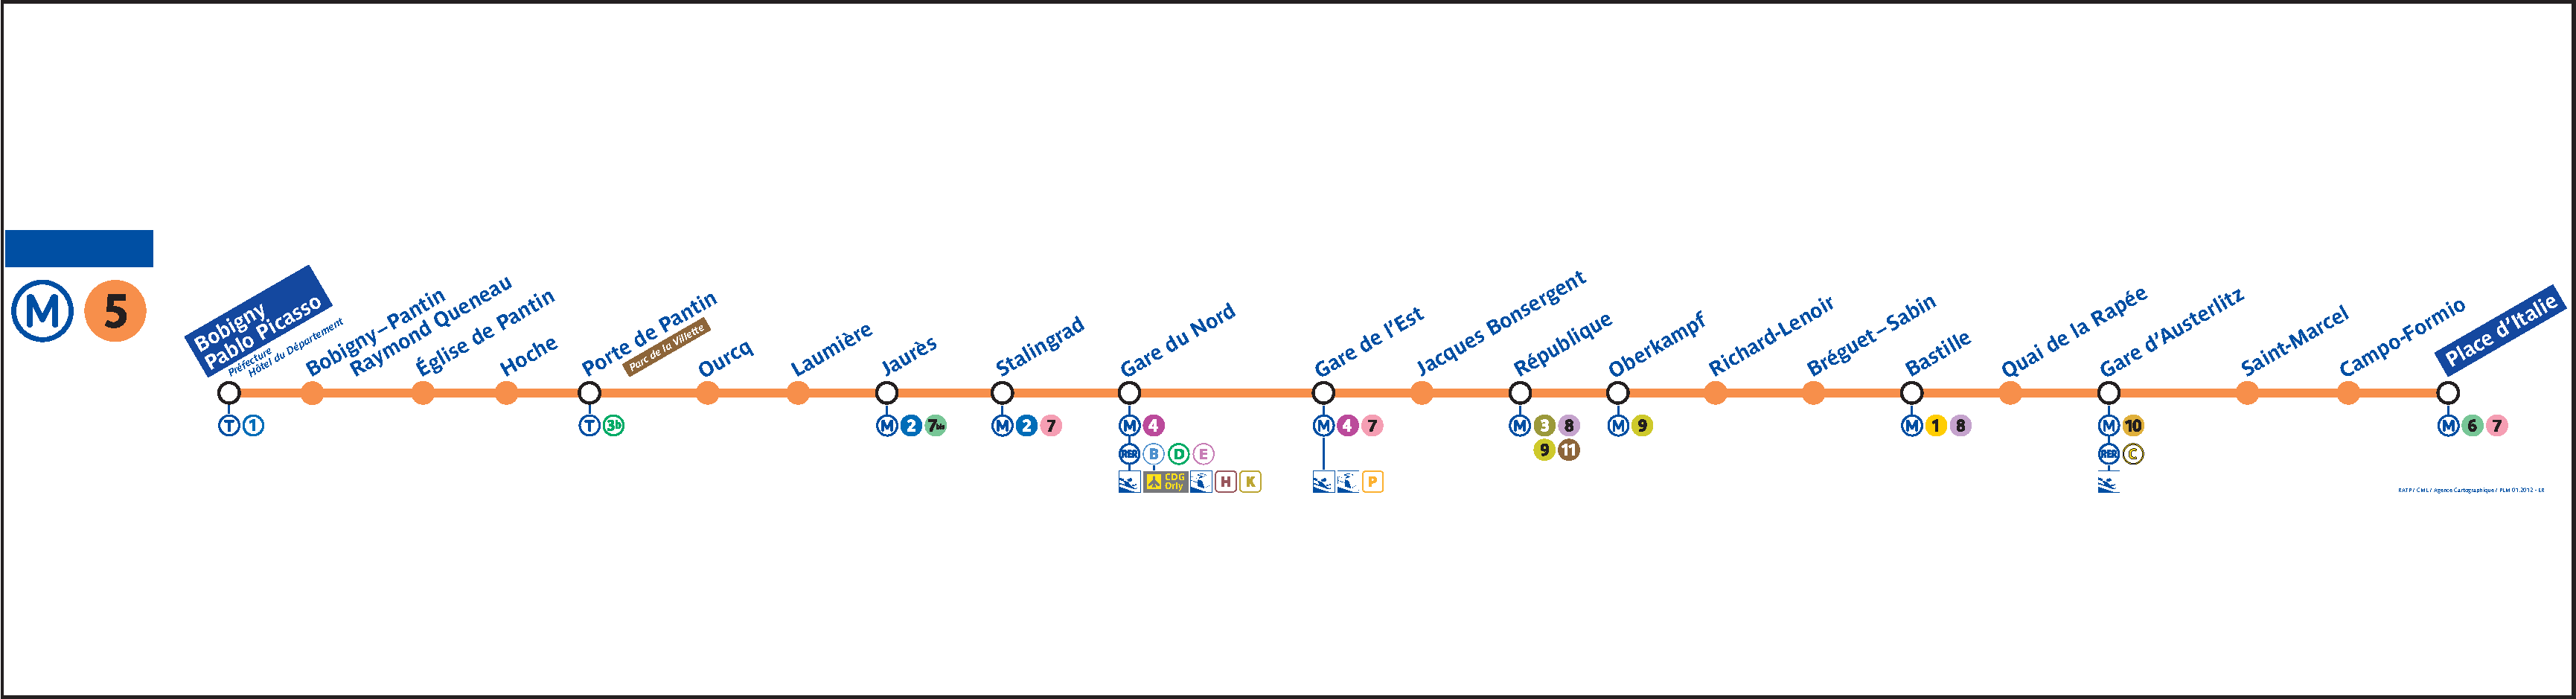
\includegraphics{img/plan_lignes/plan-de-ligne_metro_ligne-5.pdf}

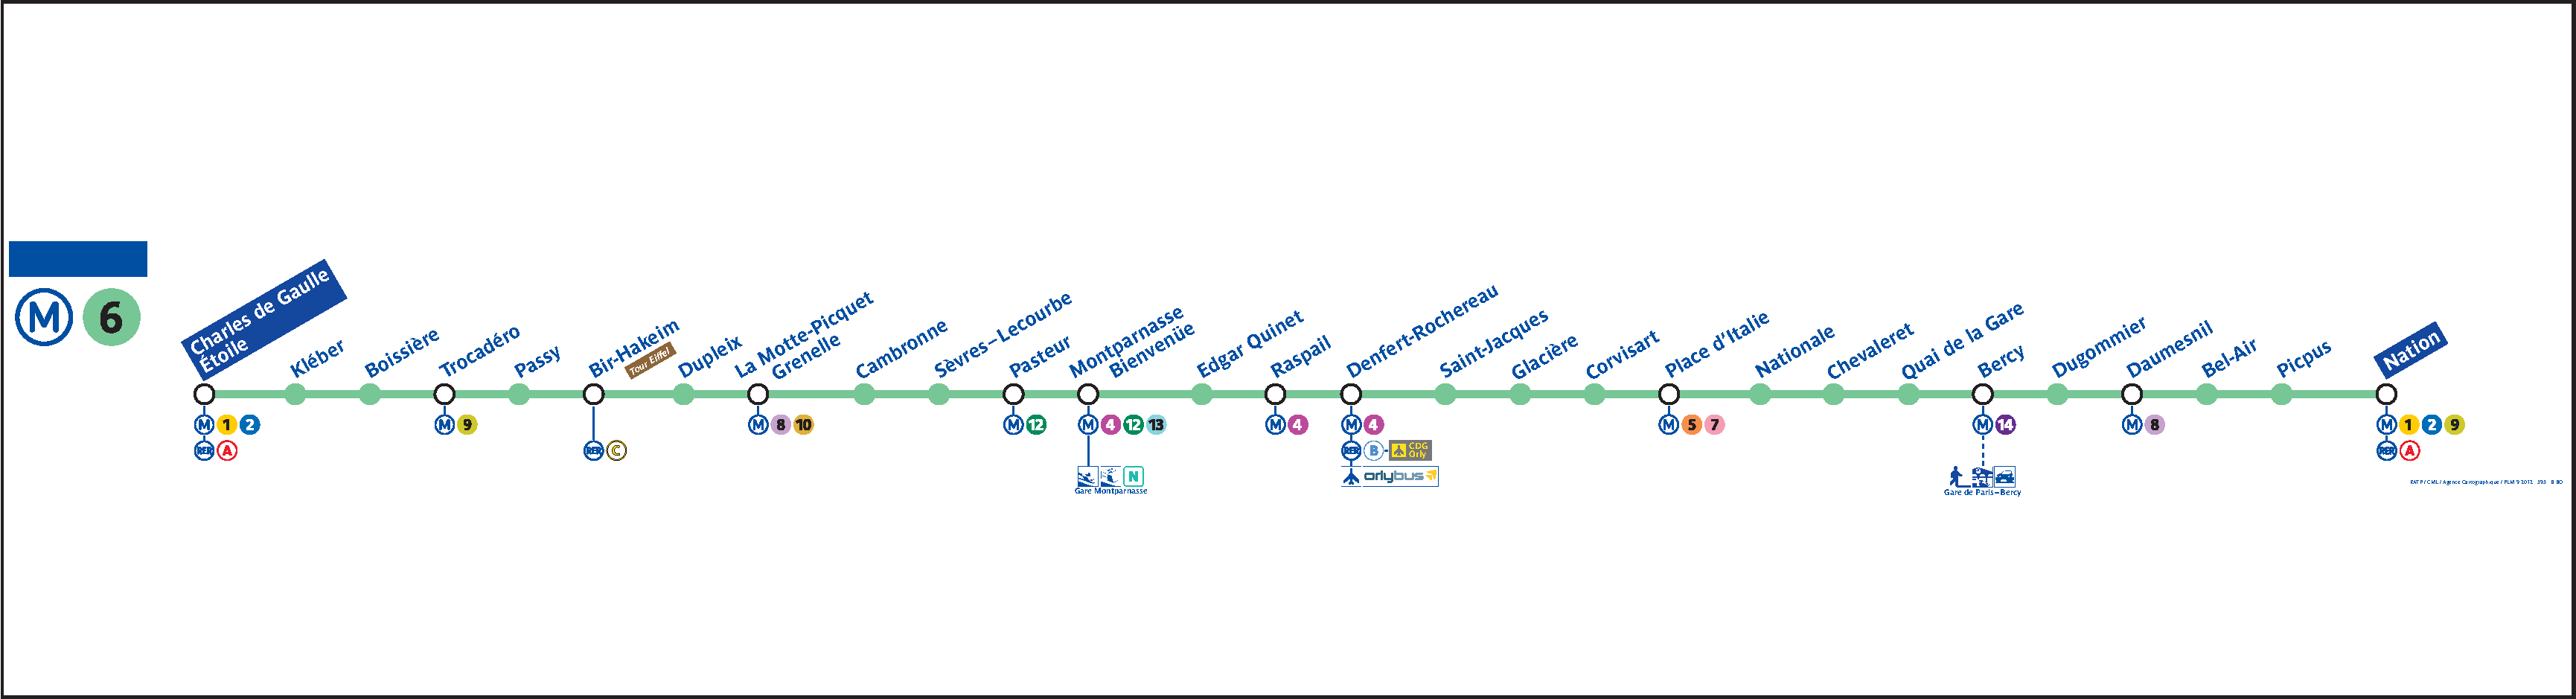
\includegraphics{img/plan_lignes/plan-de-ligne_metro_ligne-6.pdf}

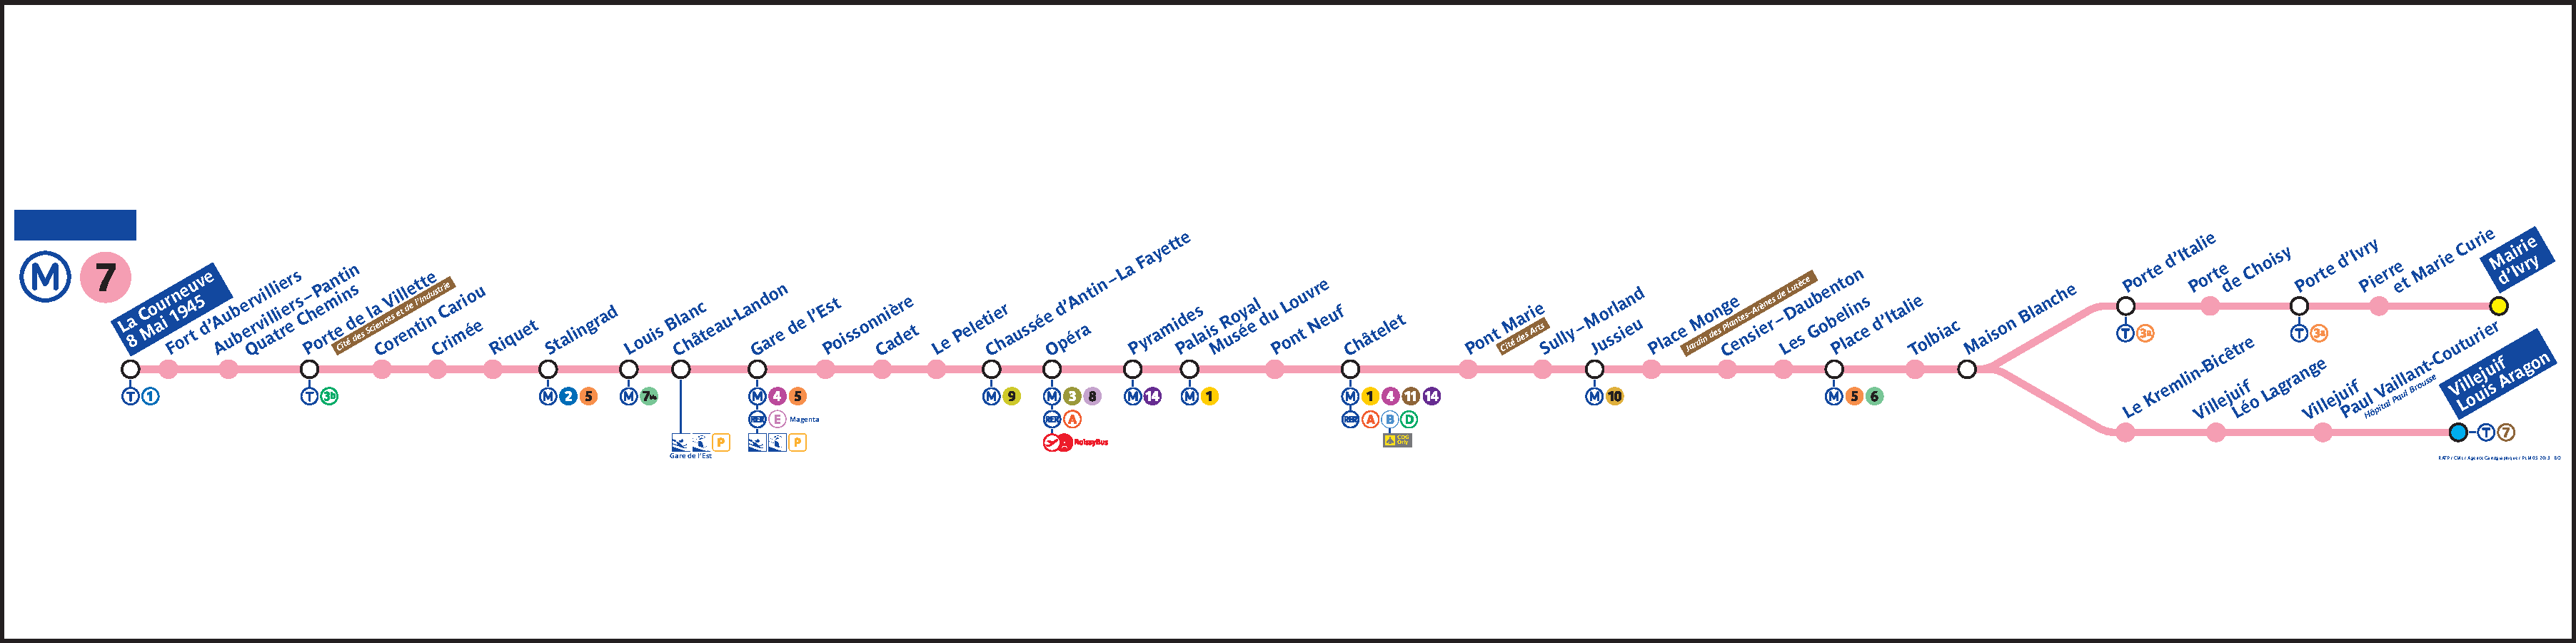
\includegraphics{img/plan_lignes/plan-de-ligne_metro_ligne-7.pdf}

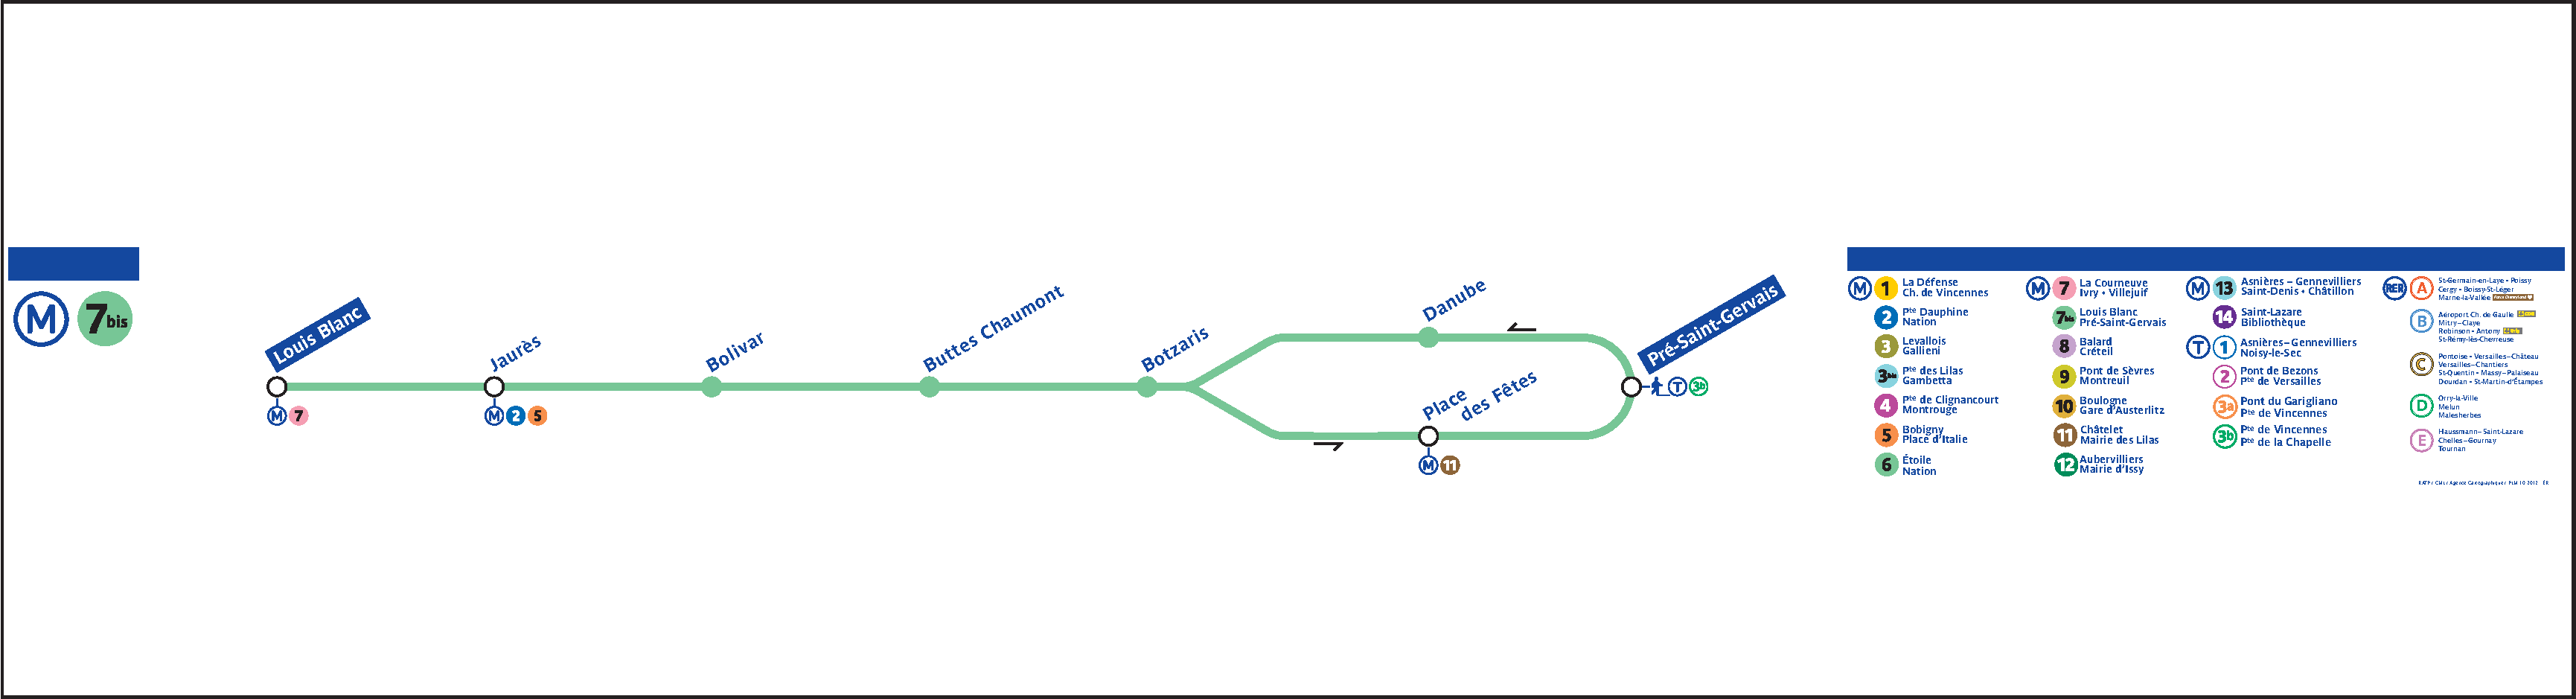
\includegraphics{img/plan_lignes/plan-de-ligne_metro_ligne-7b.pdf}

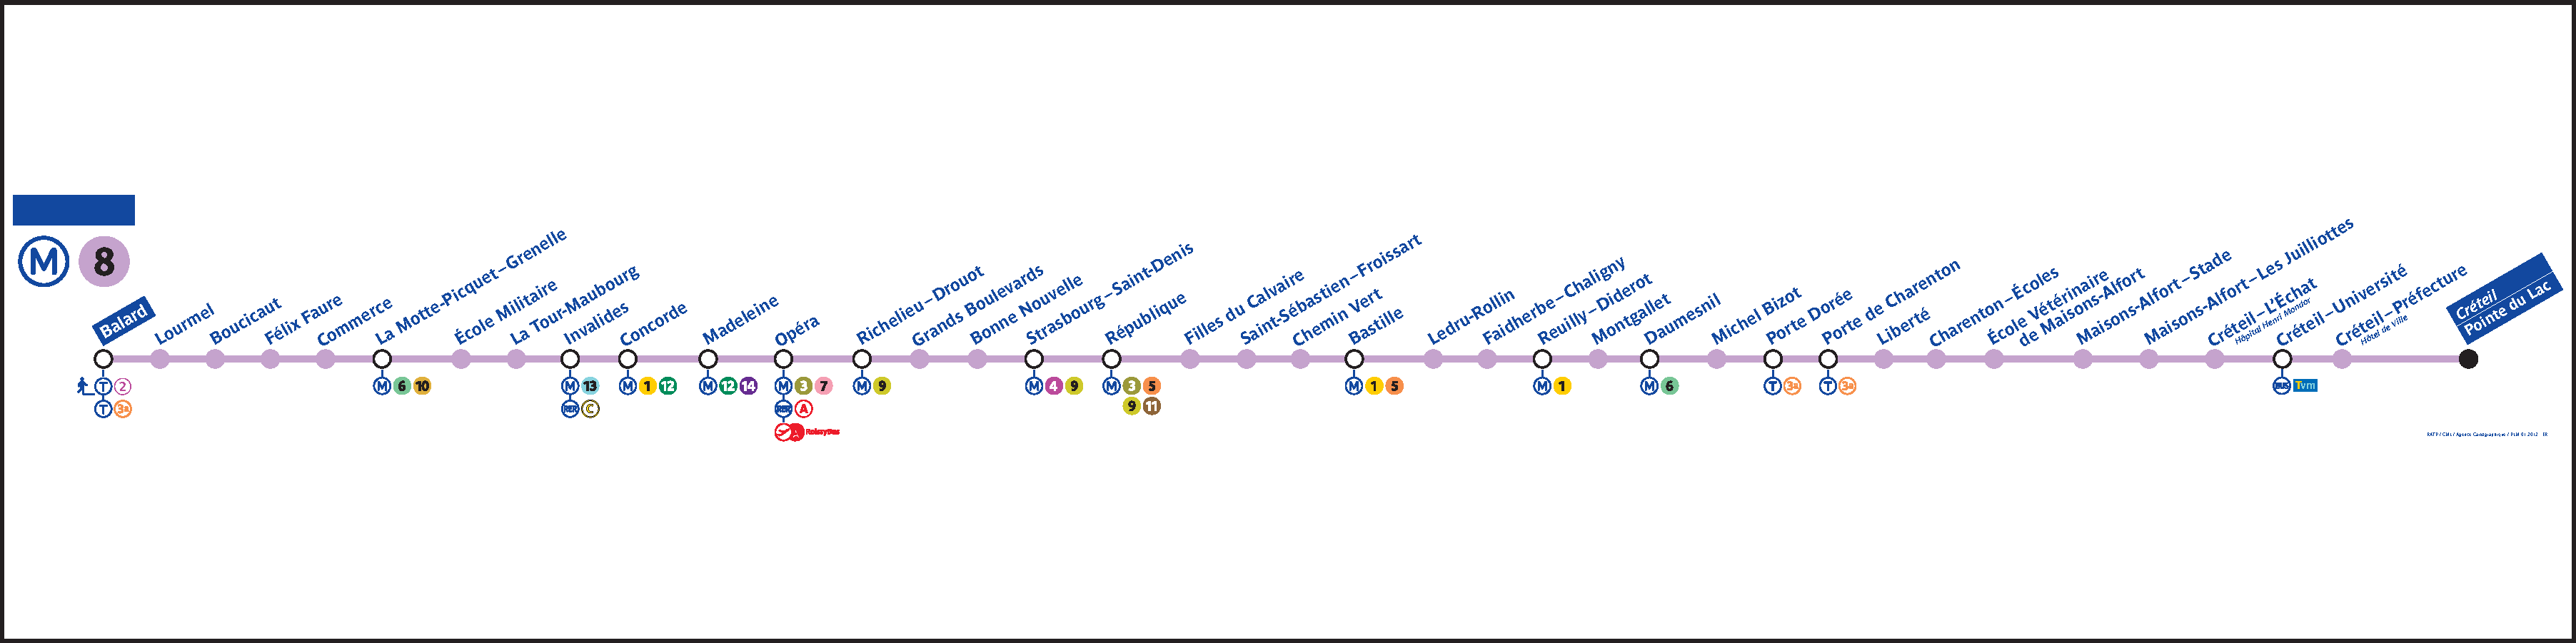
\includegraphics{img/plan_lignes/plan-de-ligne_metro_ligne-8.pdf}

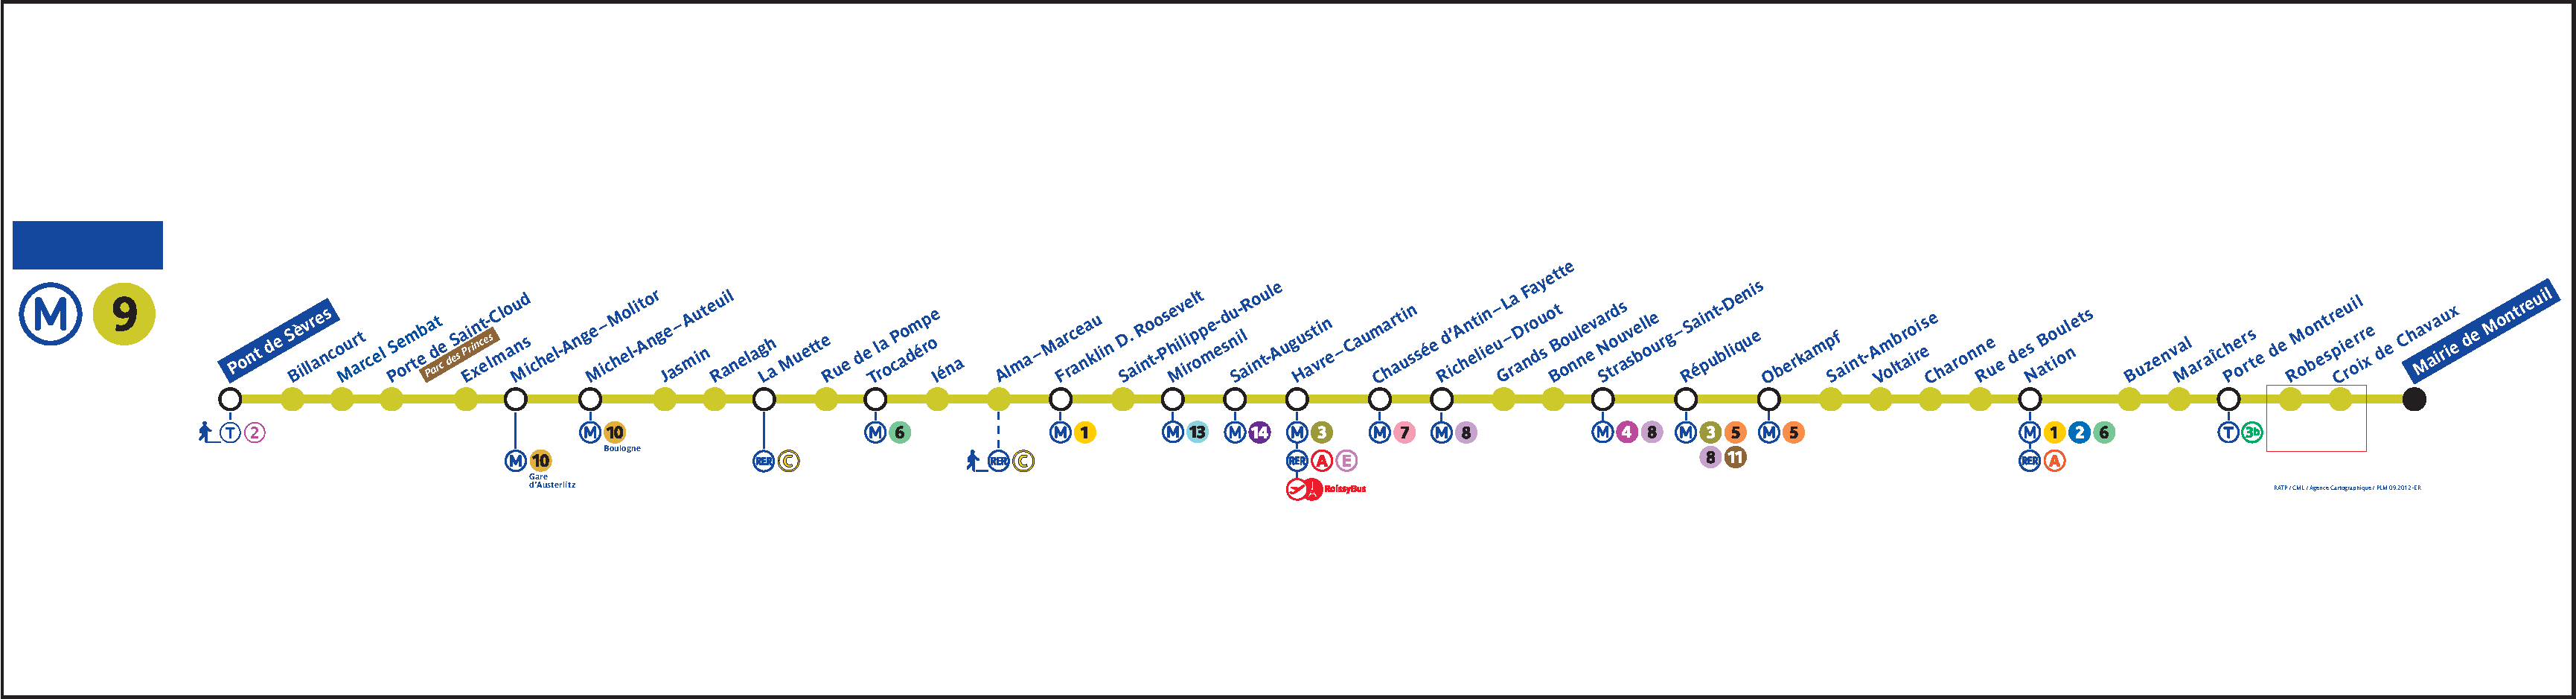
\includegraphics{img/plan_lignes/plan-de-ligne_metro_ligne-9.pdf}

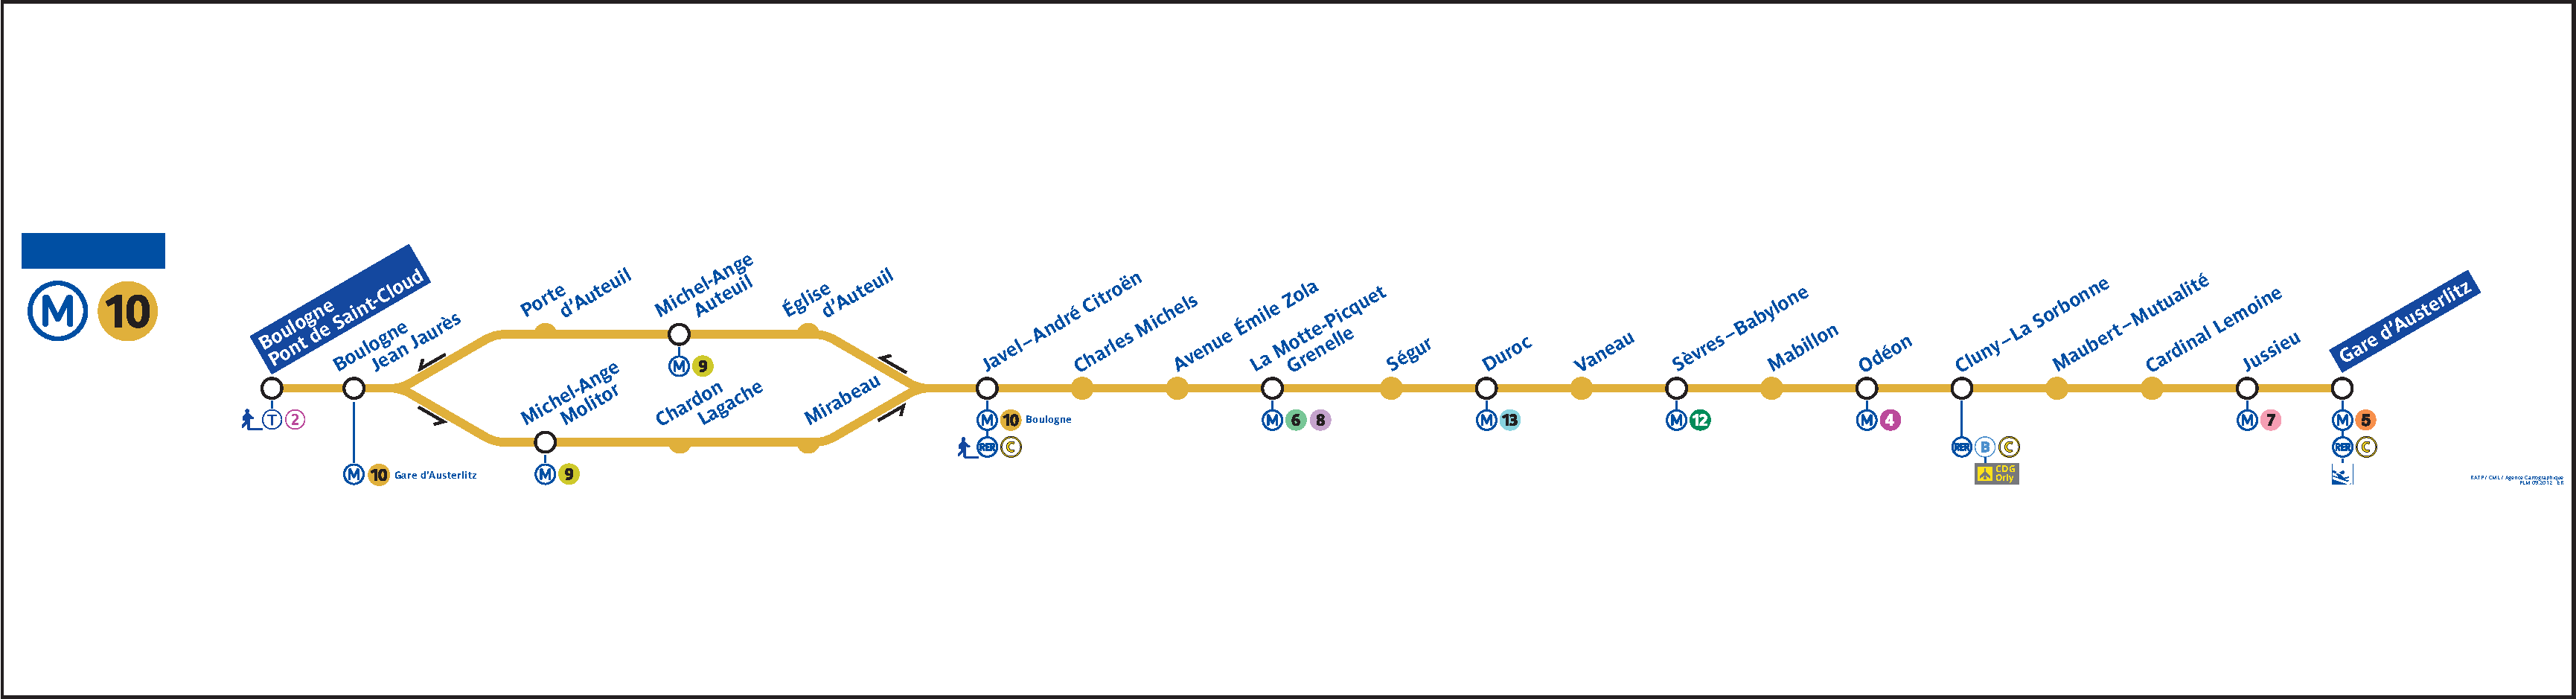
\includegraphics{img/plan_lignes/plan-de-ligne_metro_ligne-10.pdf}

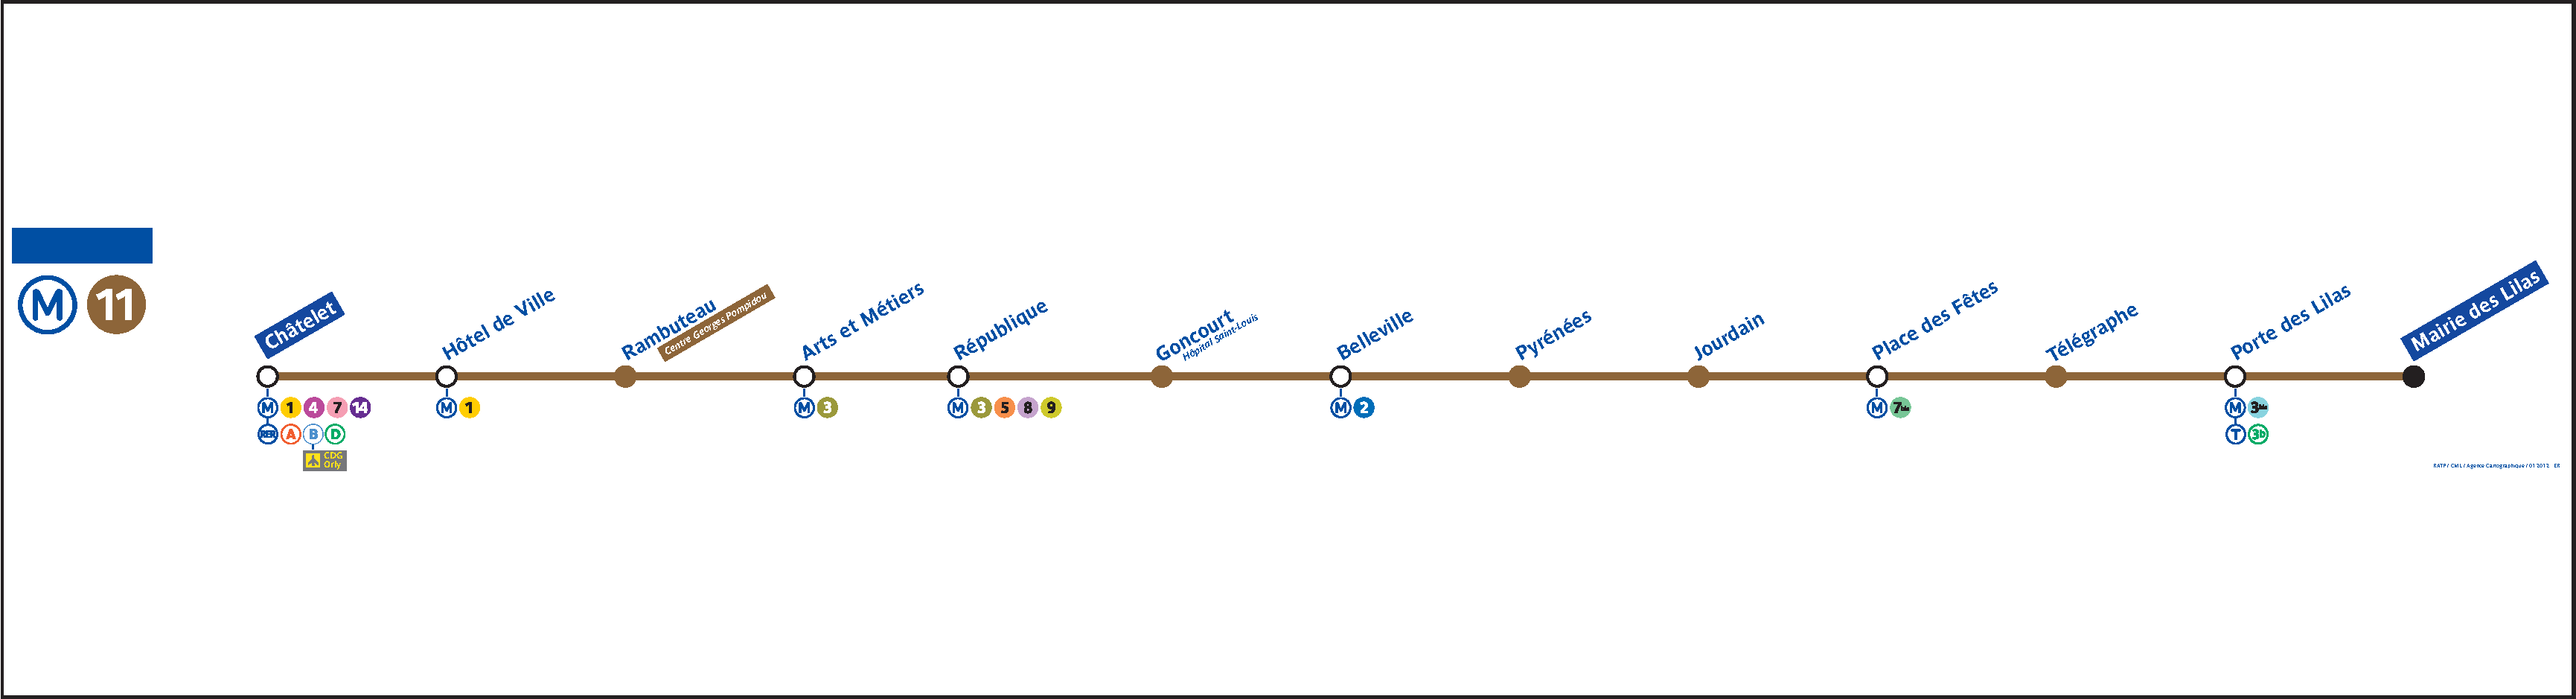
\includegraphics{img/plan_lignes/plan-de-ligne_metro_ligne-11.pdf}

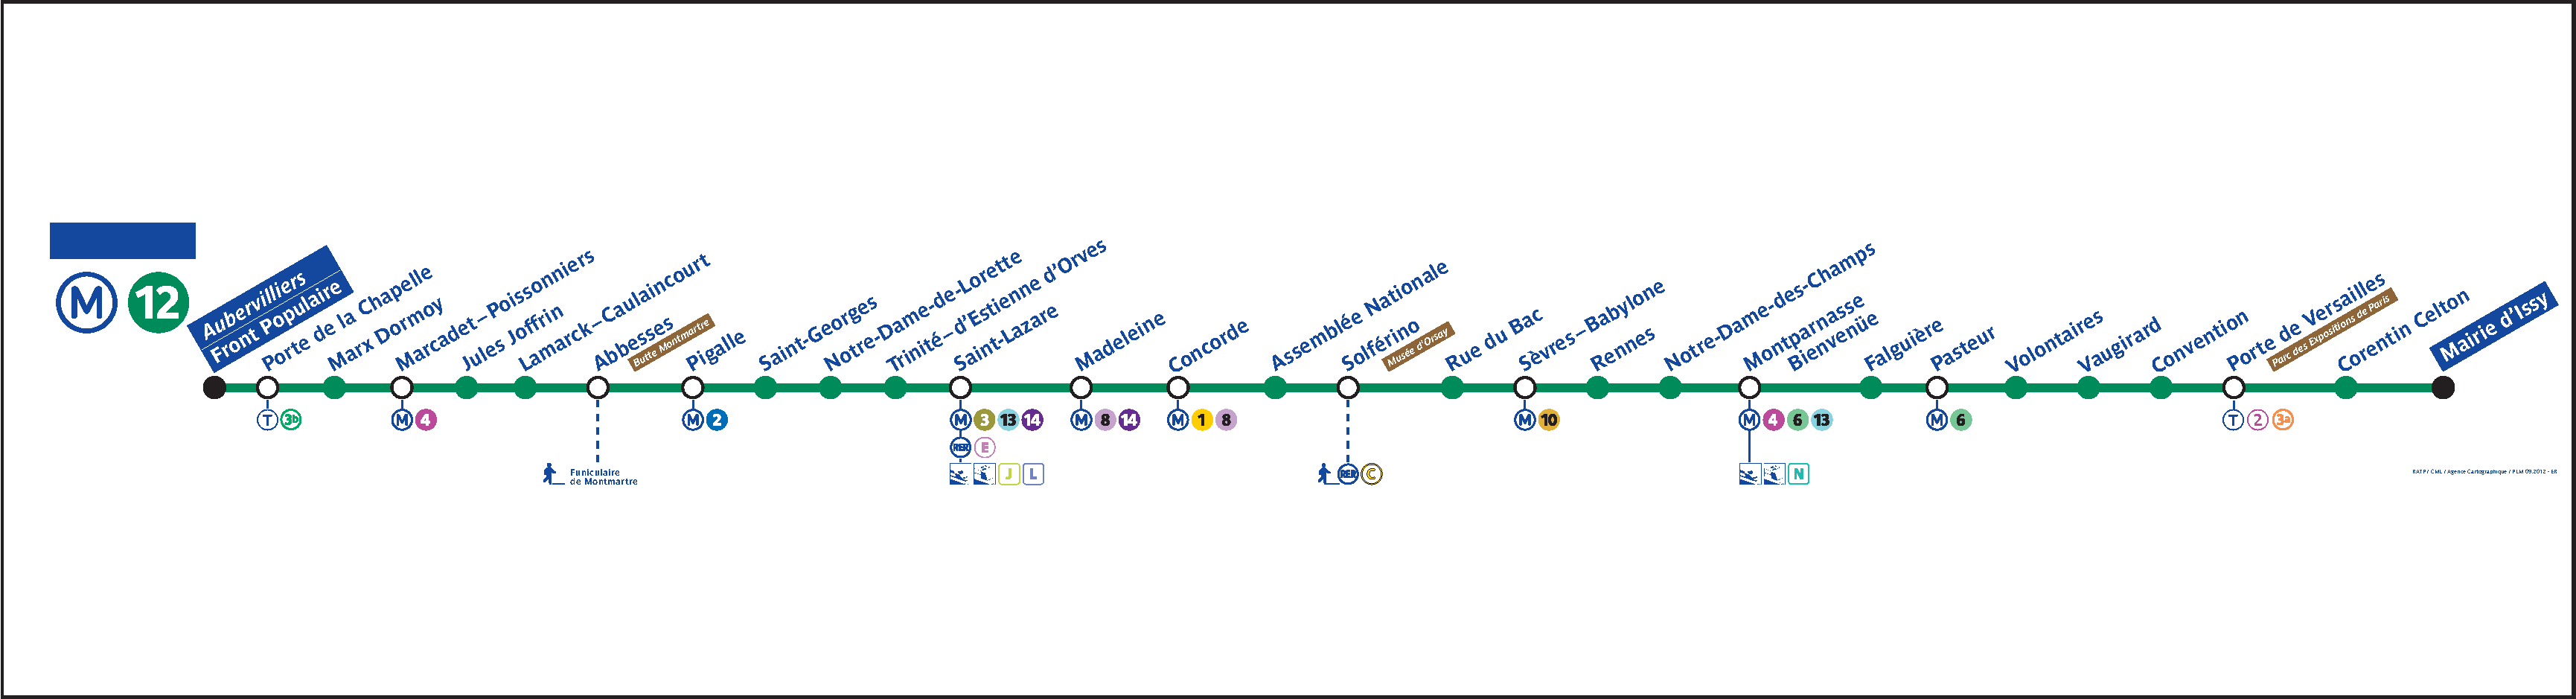
\includegraphics{img/plan_lignes/plan-de-ligne_metro_ligne-12.pdf}


\includegraphics{img/plan_lignes/plan-de-ligne_metro_ligne-13.pdf}

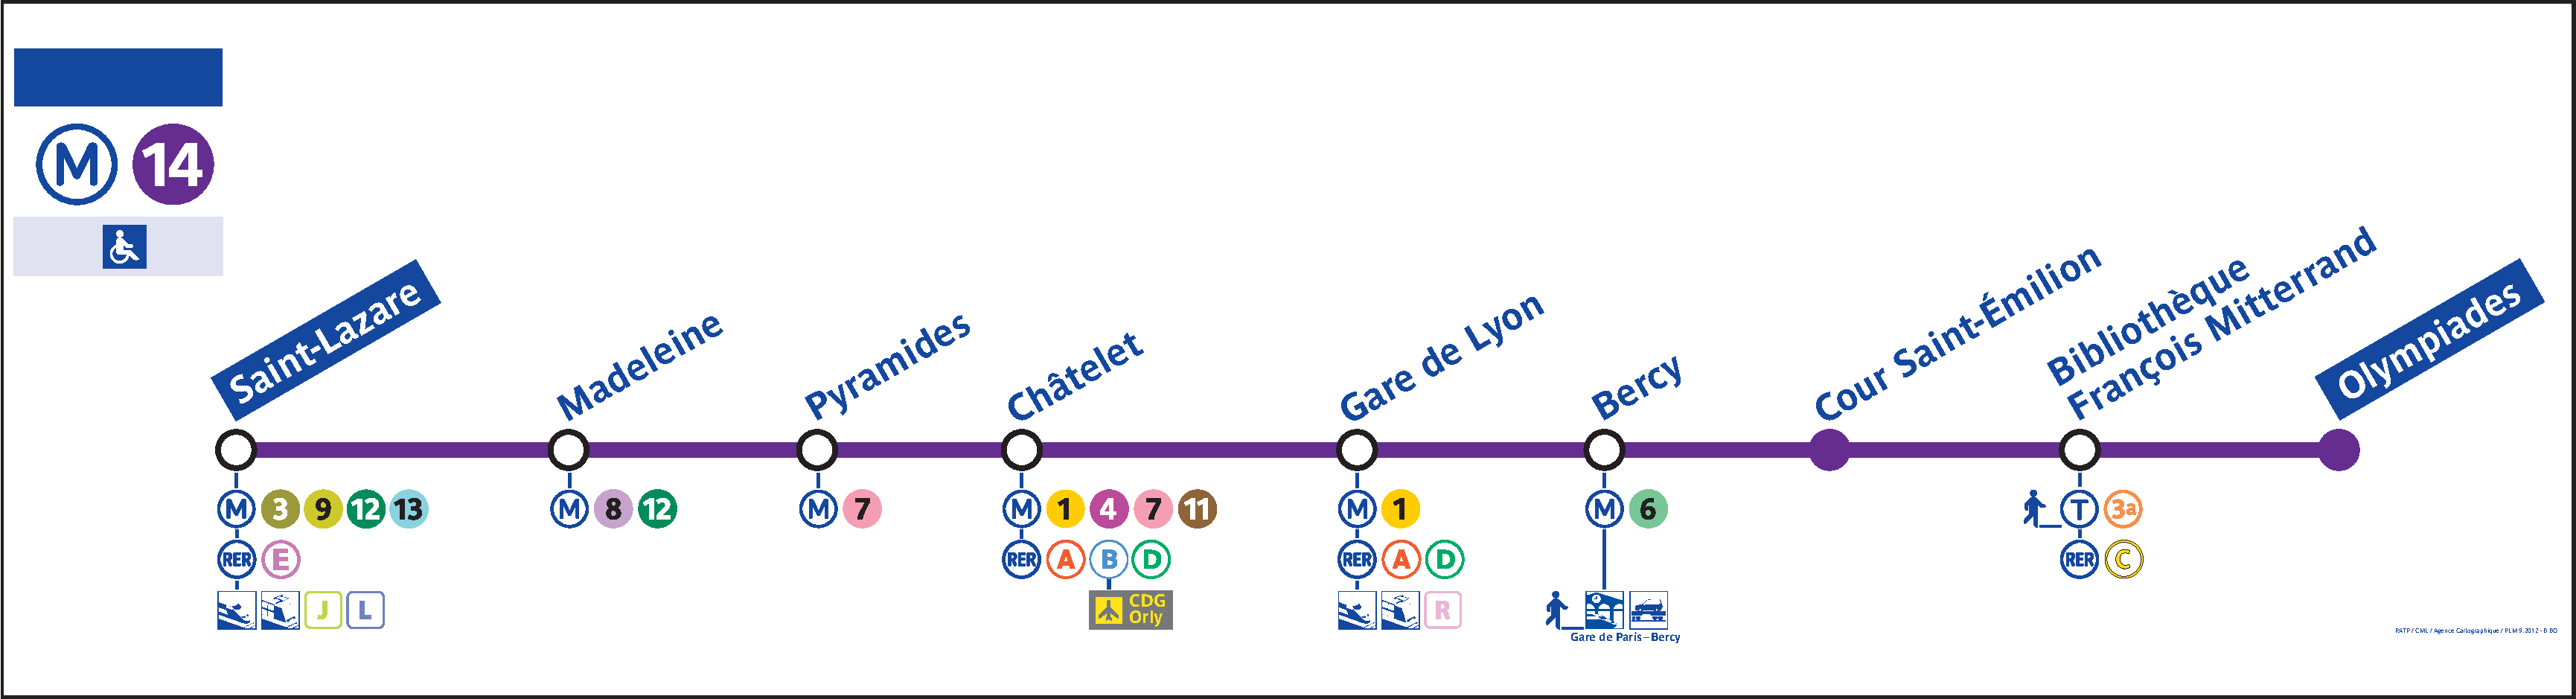
\includegraphics{img/plan_lignes/plan-de-ligne_metro_ligne-14.pdf}

\end{landscape}

\newpage

\end{document}
